\documentclass{article}
\usepackage{hyperref}
\usepackage{graphicx}
\begin{document}
\title{WebPlotDigitizer User Manual\\ Version 2.6}
\author{Ankit Rohatgi\footnote{E-Mail: ankitrohatgi@hotmail.com}}
\maketitle
\tableofcontents

\section{About}
WebPlotDigitizer is a web based software to be used for extracting numeric values from plots and figures.

\begin{figure}
\centering
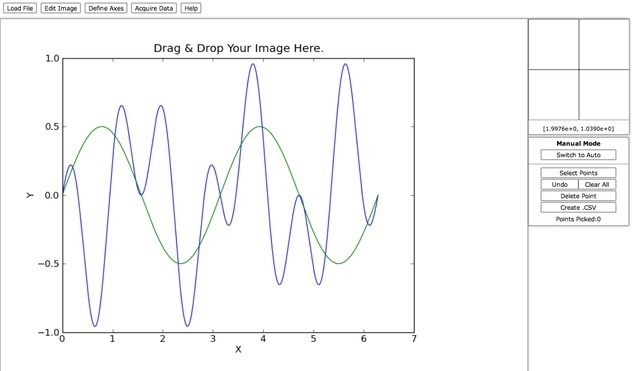
\includegraphics[width=4in]{./figures/testSmall.jpg}
\end{figure}

\section{License}
WebPlotDigitizer is distributed under GNU General Public License version 3.
\section{Availability}
Go to the website, \url{http://arohatgi.info/WebPlotDigitizer}.
\section{Supported Browsers}
Google Chrome, Mozilla Firefox, Internet Explorer 10, Safari 6.0
\section{Loading Plots}
File, Load
\end{document}
